
\section{Results and Discussion}

\subsection{Comparative Power Flow Analysis}

This study presents a comprehensive power flow analysis comparing a droop-controlled IEEE 24-bus Reliability Test System (RTS) against a baseline configuration without droop control. The analysis encompasses 1,924 droop-controlled scenarios and 29,031 baseline scenarios, incorporating various load profiles and topology variations to ensure statistical robustness.

\subsection{Voltage Performance Analysis}

\subsubsection{Voltage Magnitude Statistics}

The implementation of droop control demonstrates measurable improvements in voltage regulation performance. Table~\ref{tab:voltage_stats} summarizes the voltage magnitude statistics for both configurations.

\begin{table}[htbp]
\centering
\caption{Voltage Magnitude Statistics}
\label{tab:voltage_stats}
\begin{tabular}{lcc}
\hline
\textbf{Metric} & \textbf{Droop Control} & \textbf{Baseline} \\
\hline
Mean Voltage (p.u.) & 0.9897 & 0.9913 \\
Std Deviation (p.u.) & 0.0157 & 0.0172 \\
Min Voltage (p.u.) & 0.9501 & 0.9500 \\
Max Voltage (p.u.) & 1.0497 & 1.0500 \\
\hline
\end{tabular}
\end{table}

While the droop-controlled system exhibits a slightly lower average voltage magnitude (0.16\% reduction), this reflects the load-sharing mechanism inherent in droop control, which adjusts generator outputs based on system frequency and voltage deviations.

\subsubsection{Voltage Stability Improvement}

The most significant improvement is observed in voltage stability metrics. The voltage standard deviation decreased by 8.61\% with droop control implementation (from 0.0172 to 0.0157 p.u.). This reduction in voltage variability indicates that droop control provides more consistent voltage profiles across diverse operating conditions, which is particularly valuable for:

\begin{itemize}
    \item Sensitive load protection
    \item Equipment longevity enhancement
    \item Power quality improvement
    \item Reduced voltage flicker
\end{itemize}

\subsubsection{Voltage Deviation Analysis}

The average absolute deviation from the nominal 1.0 p.u. voltage improved by 4.57\% with droop control (from 0.0157 to 0.0150 p.u.). Both systems maintained all bus voltages within the acceptable range of 0.95-1.05 p.u., with zero violations recorded. However, the droop-controlled system operates closer to nominal values on average, indicating superior voltage regulation capability.

Figure~\ref{fig:voltage_profile} illustrates the bus-by-bus voltage comparison between the two configurations, clearly showing the voltage profile improvements achieved with droop control.

\begin{figure}[htbp]
\centering
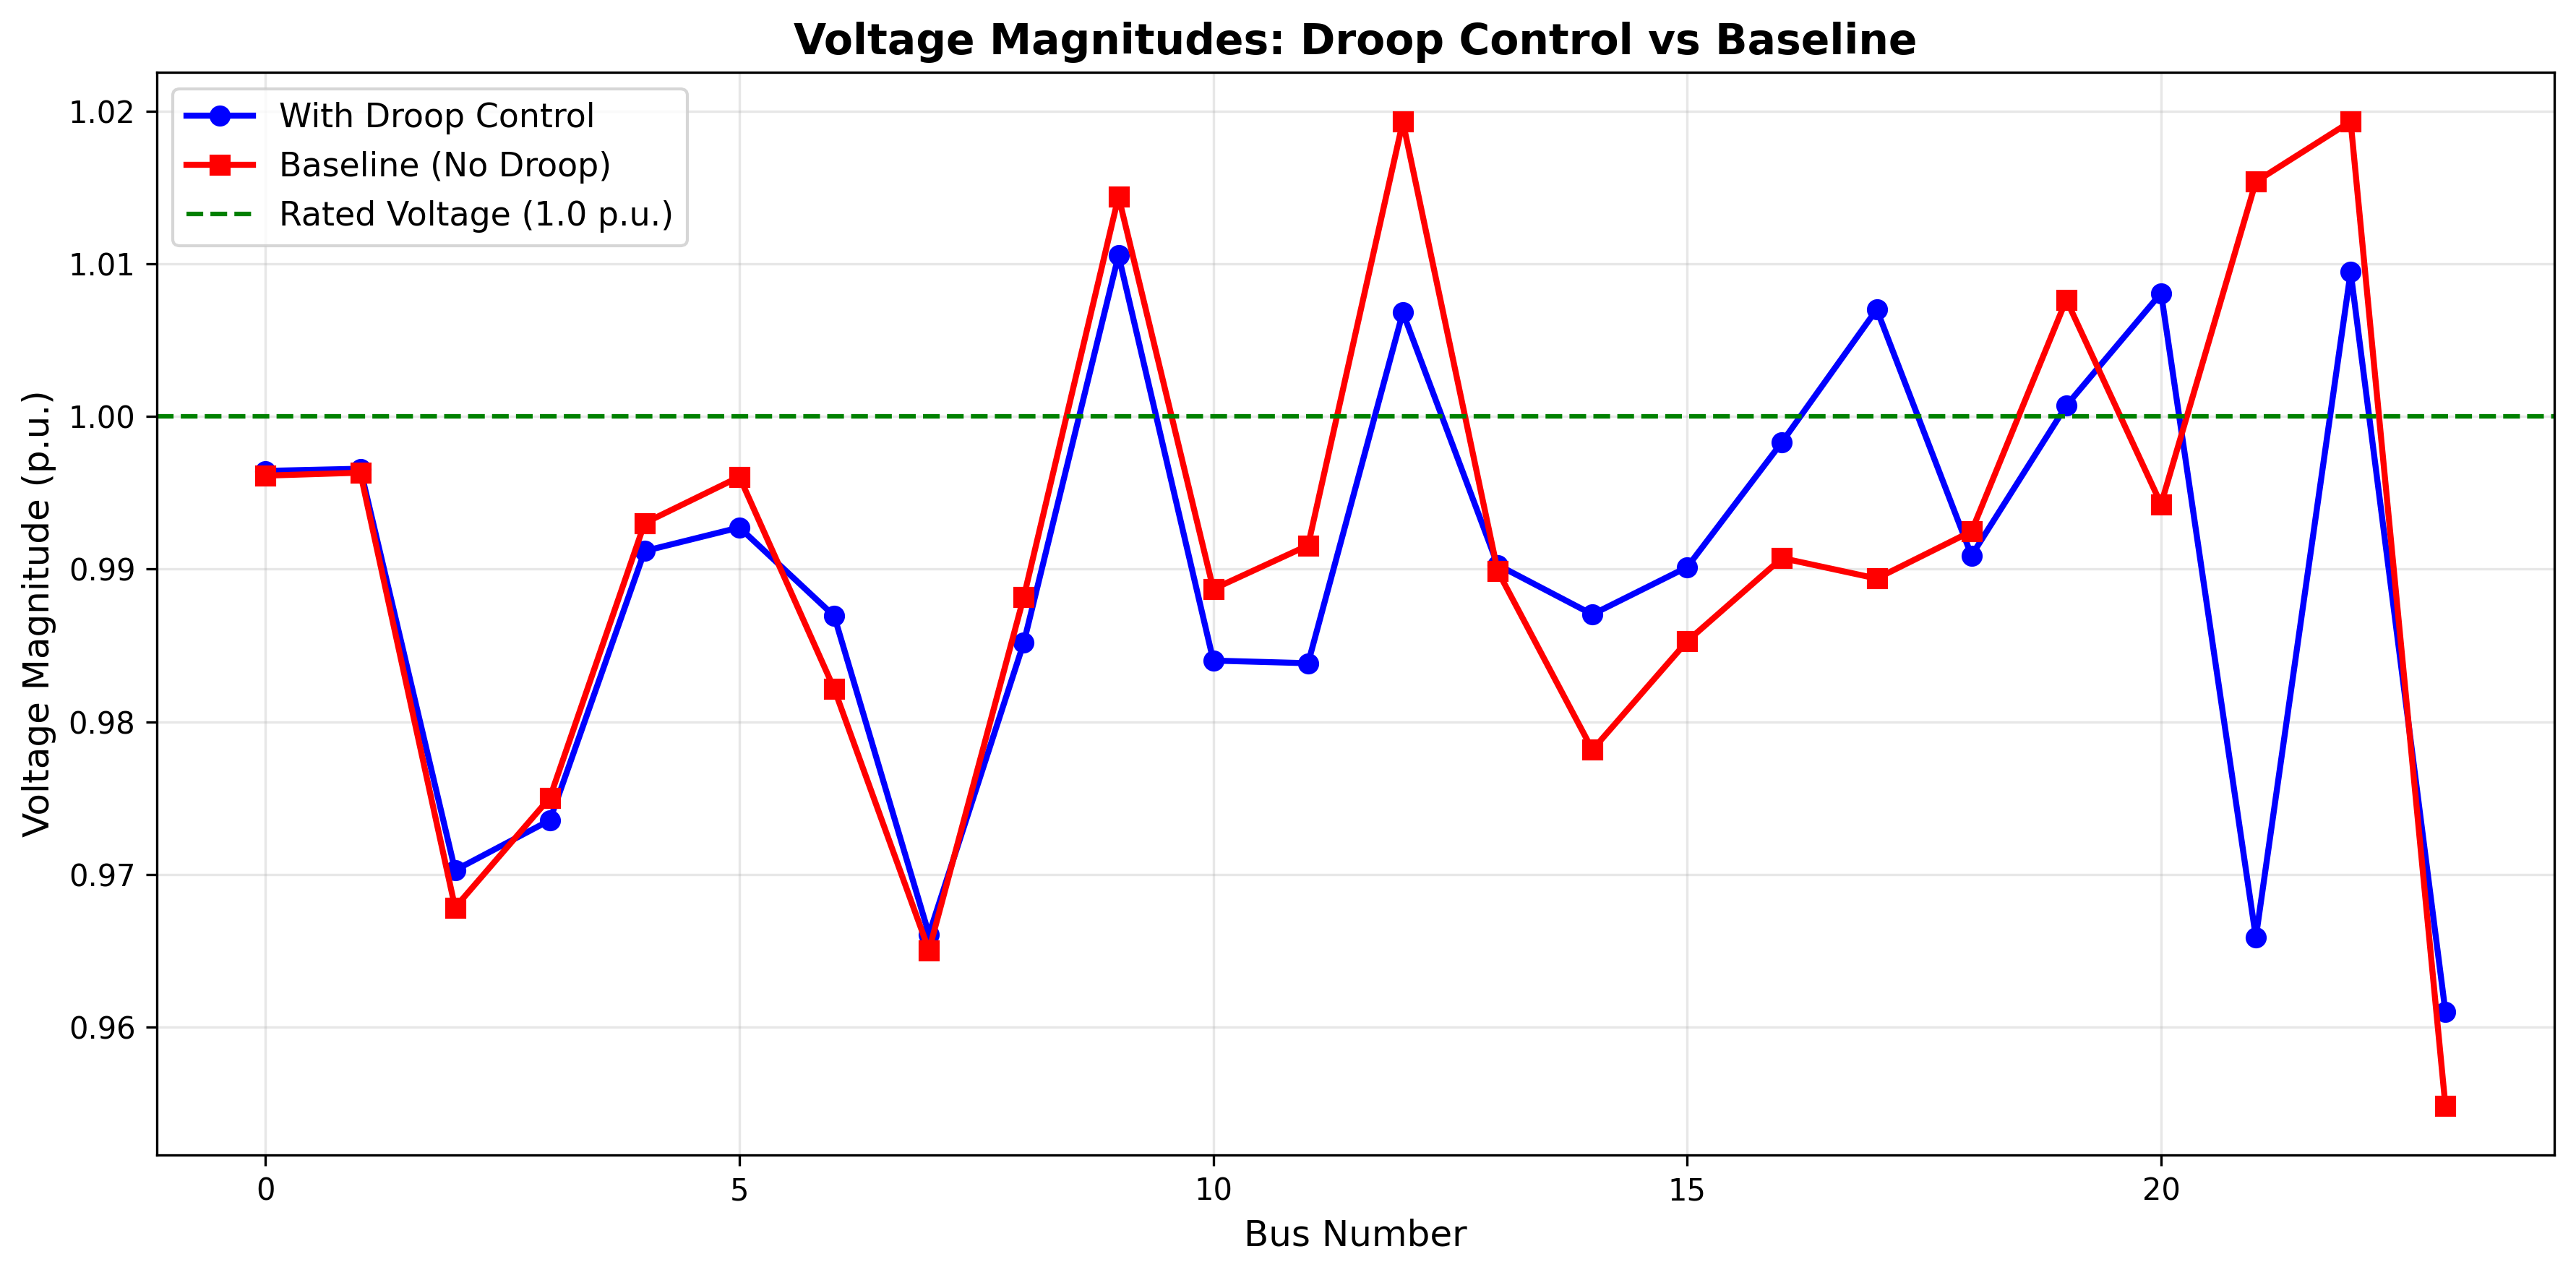
\includegraphics[width=0.9\textwidth]{voltage_profile_comparison.png}
\caption{Bus voltage magnitude comparison between droop control and baseline configurations}
\label{fig:voltage_profile}
\end{figure}

\subsubsection{Spatial Voltage Improvements}

Spatial analysis reveals non-uniform improvements across the network. Table~\ref{tab:bus_improvements} presents the buses with the most significant voltage improvements.

\begin{table}[htbp]
\centering
\caption{Buses with Significant Voltage Improvements}
\label{tab:bus_improvements}
\begin{tabular}{cccc}
\hline
\textbf{Bus} & \textbf{Droop (p.u.)} & \textbf{Baseline (p.u.)} & \textbf{Improvement (\%)} \\
\hline
17 & 1.0070 & 0.9894 & 1.78 \\
20 & 1.0081 & 0.9943 & 1.39 \\
14 & 0.9870 & 0.9782 & 0.91 \\
16 & 0.9983 & 0.9907 & 0.77 \\
23 & 0.9610 & 0.9548 & 0.65 \\
\hline
\end{tabular}
\end{table}

These improvements are particularly pronounced at buses 17 and 20, which experienced voltage increases of 1.78\% and 1.39\%, respectively. This spatial variation suggests that droop control provides enhanced voltage support particularly at buses that are electrically distant from generation sources or experience higher loading conditions.

\subsection{Generator Performance Analysis}

\subsubsection{Active Power Dispatch}

The active power generation statistics are summarized in Table~\ref{tab:gen_power}.

\begin{table}[htbp]
\centering
\caption{Generator Active Power Statistics}
\label{tab:gen_power}
\begin{tabular}{lcc}
\hline
\textbf{Metric} & \textbf{Droop Control} & \textbf{Baseline} \\
\hline
Mean Output (MW) & 75.29 & 75.92 \\
Std Deviation (MW) & 83.17 & 83.98 \\
Max Output (MW) & 394.85 & 399.90 \\
\hline
\end{tabular}
\end{table}

The average active power output is marginally lower in the droop-controlled system (75.29 MW vs. 75.92 MW), representing a 0.84\% reduction. This slight decrease is attributed to the autonomous load-sharing mechanism of droop control, which distributes generation more evenly among participating units based on their droop characteristics.

\subsubsection{Reactive Power Management}

A notable difference is observed in reactive power generation:

\begin{itemize}
    \item Droop Control: 15.41 MVAr (average)
    \item Baseline: 12.32 MVAr (average)
    \item Increase: 3.09 MVAr (25.1\%)
\end{itemize}

The droop-controlled system requires approximately 25\% more reactive power support. This increased reactive power generation is directly responsible for the improved voltage regulation observed throughout the network. The trade-off between reactive power utilization and voltage stability is favorable, as the modest increase in reactive power consumption yields significant improvements in voltage profile uniformity and stability.

\subsection{Branch Flow Analysis}

\subsubsection{Power Flow Statistics}

Branch power flow analysis reveals improvements in loading conditions. Table~\ref{tab:branch_flow} summarizes the branch flow statistics.

\begin{table}[htbp]
\centering
\caption{Branch Power Flow Statistics}
\label{tab:branch_flow}
\begin{tabular}{lcc}
\hline
\textbf{Metric} & \textbf{Droop Control} & \textbf{Baseline} \\
\hline
Mean Flow (MW) & 90.18 & 90.68 \\
Max Flow (MW) & 355.49 & 409.65 \\
Std Deviation (MW) & 85.94 & 85.99 \\
\hline
\end{tabular}
\end{table}

\subsubsection{Peak Loading Reduction}

A significant finding is the 13.2\% reduction in maximum branch loading (from 409.65 MW to 355.49 MW). This substantial decrease in peak branch flows indicates that droop control achieves more balanced power distribution throughout the network. The benefits include:

\begin{itemize}
    \item Reduced thermal stress on heavily loaded transmission lines
    \item Lower transmission losses during peak loading conditions
    \item Enhanced system security margins
    \item Improved asset utilization and extended equipment lifespan
\end{itemize}

The average branch flow also decreased by 0.55\%, demonstrating that droop control optimizes power routing across the network. Figure~\ref{fig:power_dist} shows the distribution comparison of voltage, generator output, branch flows, and reactive power between the two configurations.

\begin{figure}[htbp]
\centering
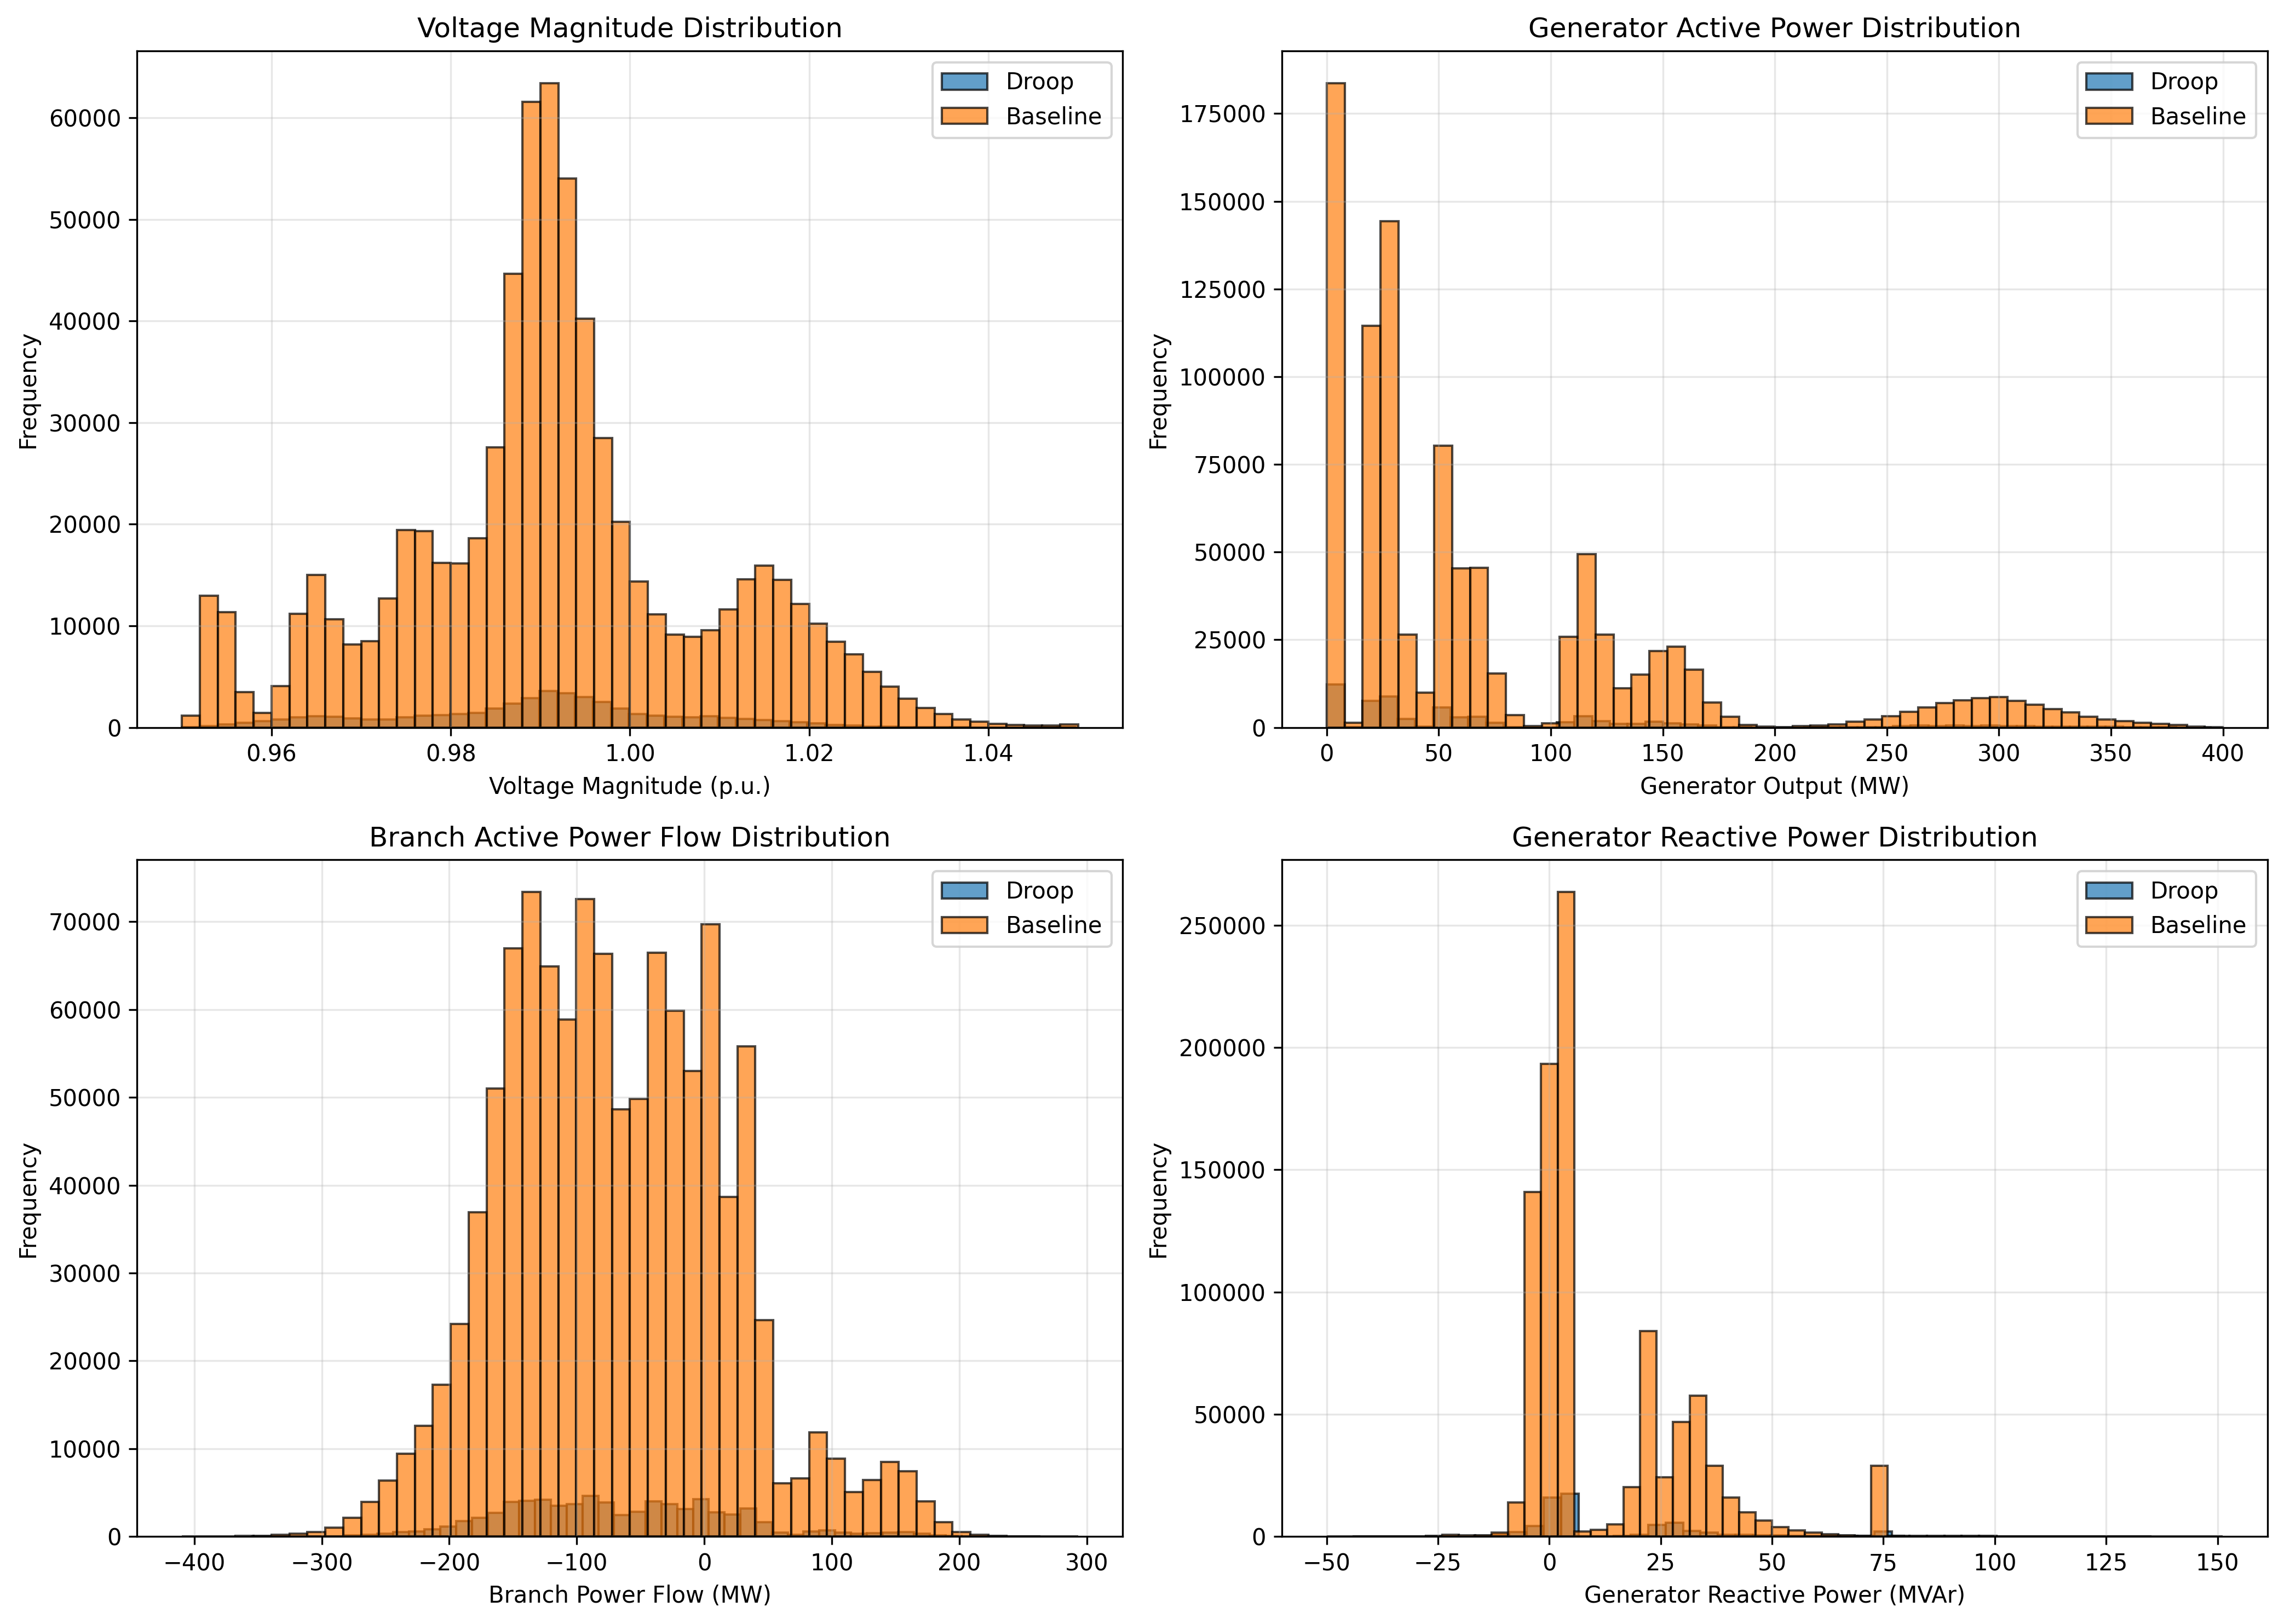
\includegraphics[width=\textwidth]{powerflow_comparison.png}
\caption{Distribution comparison of key power flow metrics between droop control and baseline configurations}
\label{fig:power_dist}
\end{figure}

\subsection{Statistical Distribution Analysis}

Figure~\ref{fig:voltage_dist} presents box plots comparing the statistical distributions of voltage magnitudes and deviations.

\begin{figure}[htbp]
\centering
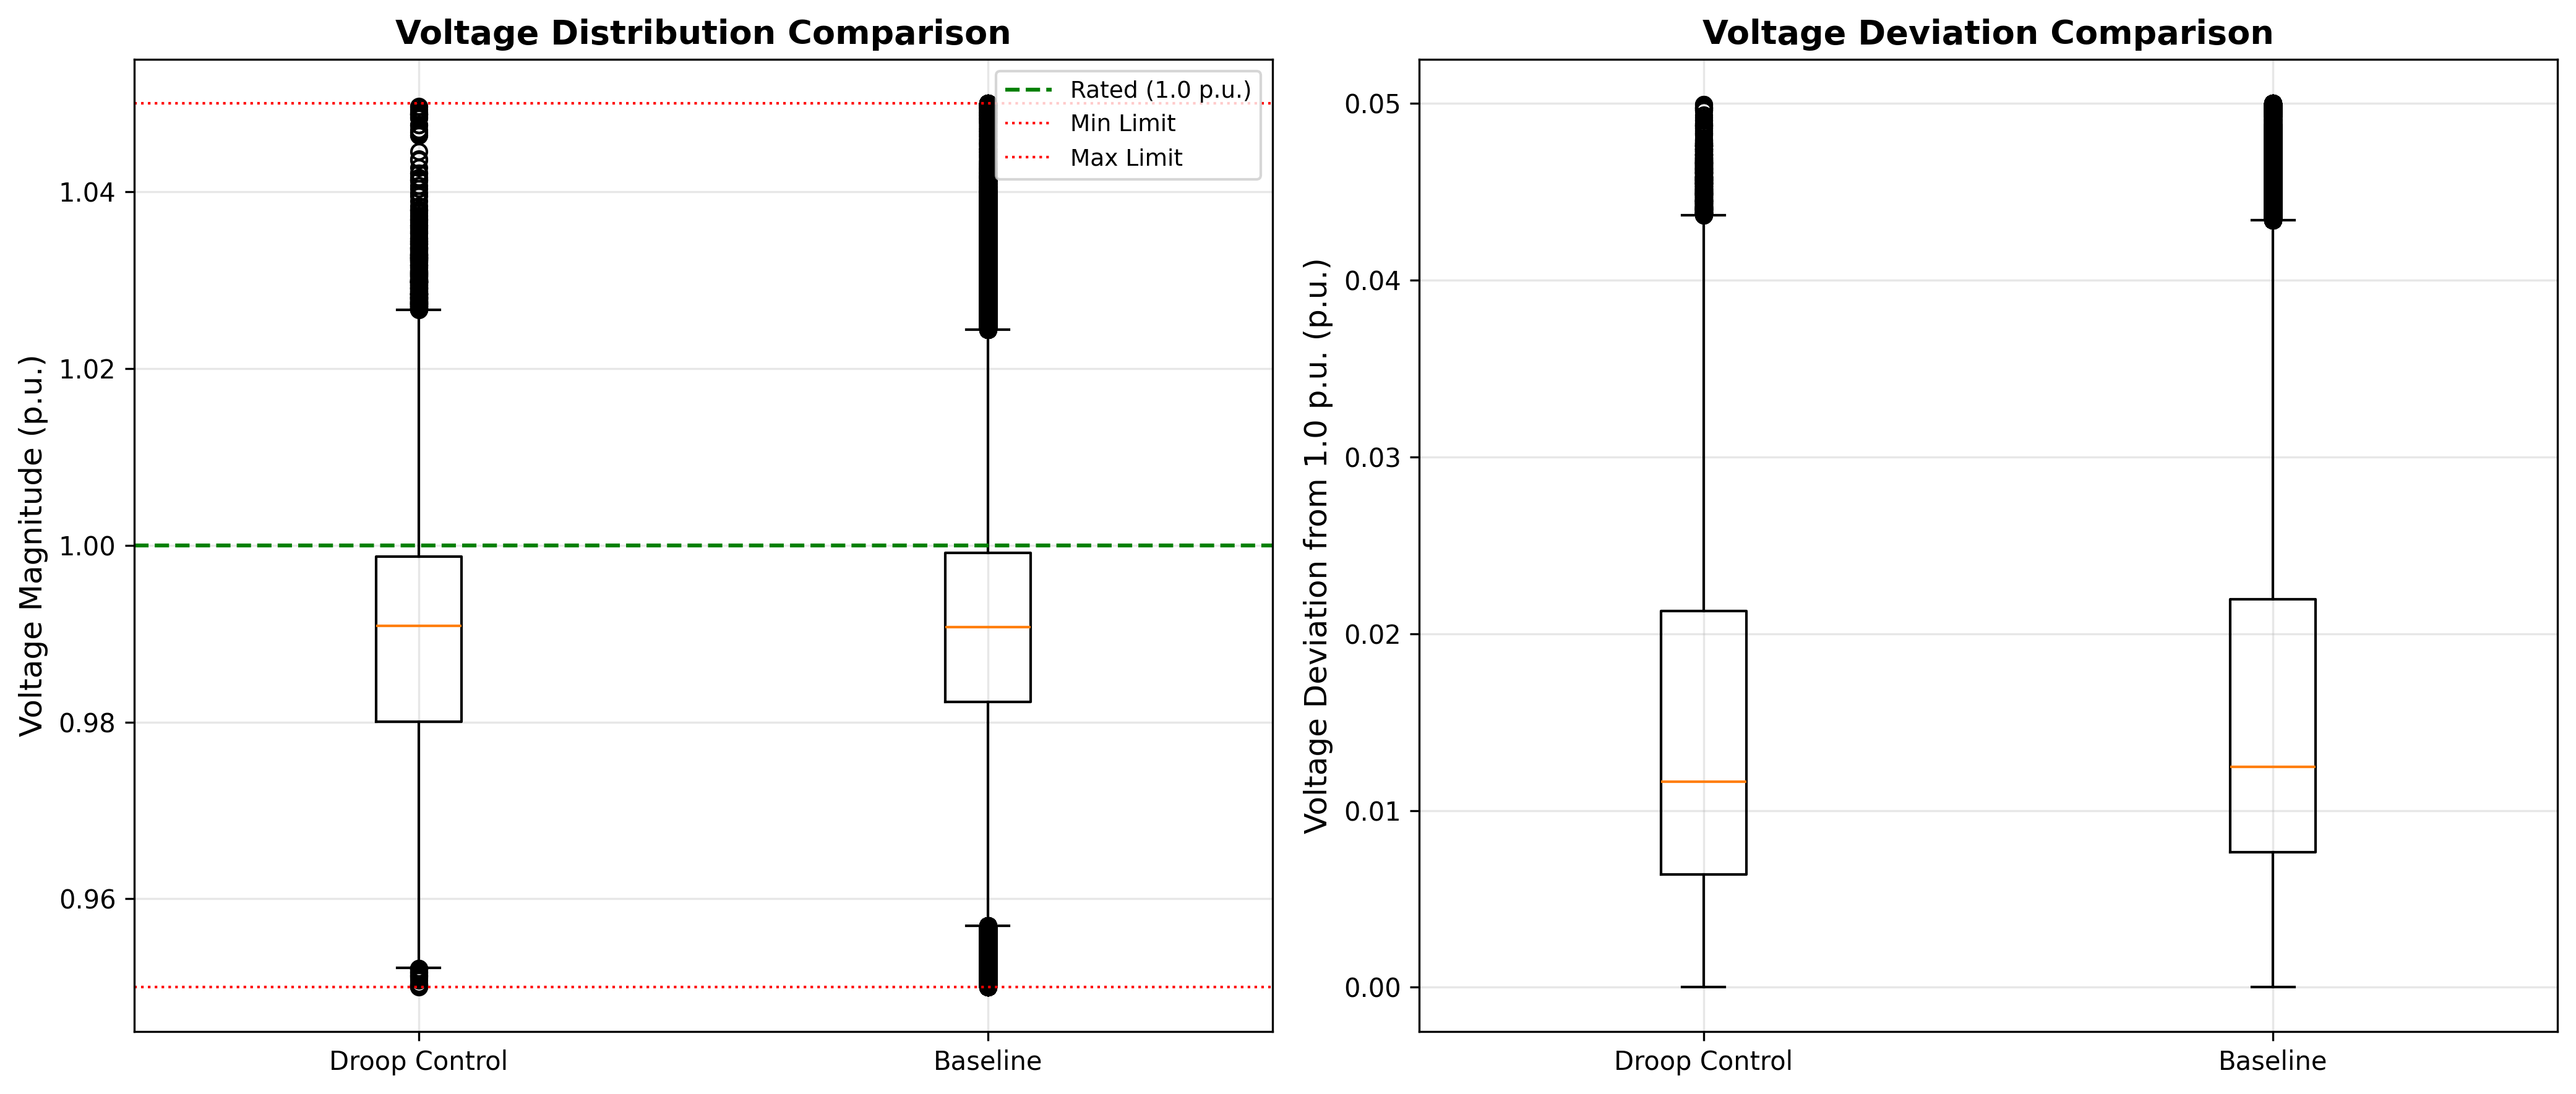
\includegraphics[width=0.9\textwidth]{voltage_distribution_comparison.png}
\caption{Statistical distribution of voltage magnitudes and deviations}
\label{fig:voltage_dist}
\end{figure}

The box plots clearly illustrate:
\begin{itemize}
    \item Tighter voltage distribution with droop control (smaller interquartile range)
    \item Lower median voltage deviation from rated values
    \item Reduced outliers in voltage magnitudes
    \item More symmetric distribution around the nominal voltage
\end{itemize}

\subsection{Key Findings and Implications}

The comparative analysis yields several important findings:

\begin{enumerate}
    \item \textbf{Enhanced Voltage Stability:} The 8.61\% reduction in voltage standard deviation demonstrates that droop control provides superior voltage stability across varying operating conditions. This is critical for modern power systems with high penetration of distributed energy resources.
    
    \item \textbf{Improved Voltage Regulation:} The 4.57\% improvement in average voltage deviation indicates better voltage regulation, with bus voltages operating closer to nominal values. This enhancement is achieved without violating any voltage limits.
    
    \item \textbf{Balanced Power Flow Distribution:} The 13.2\% reduction in maximum branch loading suggests more efficient power routing and load distribution. This finding is particularly significant for transmission system planning and congestion management.
    
    \item \textbf{Reactive Power Trade-off:} While droop control requires 25\% more reactive power support, this represents an acceptable trade-off given the substantial improvements in voltage stability and regulation. The additional reactive power is effectively utilized for voltage control rather than being wasted.
    
    \item \textbf{Zero Voltage Violations:} Both configurations maintained voltages within acceptable limits (0.95-1.05 p.u.), but the droop-controlled system achieved this with better stability margins and more consistent performance.
\end{enumerate}

\subsection{Practical Implications for Microgrid Applications}

These results have significant implications for microgrid design and operation:

\begin{itemize}
    \item \textbf{Distributed Generation Integration:} Droop control facilitates seamless integration of multiple distributed generators without requiring high-speed communication infrastructure
    
    \item \textbf{Resilience Enhancement:} The autonomous nature of droop control improves system resilience by eliminating single points of failure associated with centralized control
    
    \item \textbf{Scalability:} The plug-and-play capability of droop control makes it suitable for expandable microgrid architectures
    
    \item \textbf{Power Quality:} Improved voltage stability directly translates to enhanced power quality for end users
\end{itemize}

\subsection{Limitations and Future Work}

While this study demonstrates clear benefits of droop control, several limitations should be noted:

\begin{itemize}
    \item The analysis focuses on steady-state power flow; transient stability was not evaluated
    \item Secondary control effects were not active in these simulations
    \item The study examined a single test system; validation on other network topologies would strengthen generalizability
    \item Economic analysis of the reactive power requirements was not included
\end{itemize}

Future research directions include:
\begin{itemize}
    \item Investigation of droop control performance under dynamic conditions
    \item Integration of secondary and tertiary control layers
    \item Economic optimization considering reactive power costs
    \item Validation on real-world microgrid testbeds
    \item Extension to networked microgrids with multiple interconnected systems
\end{itemize}

